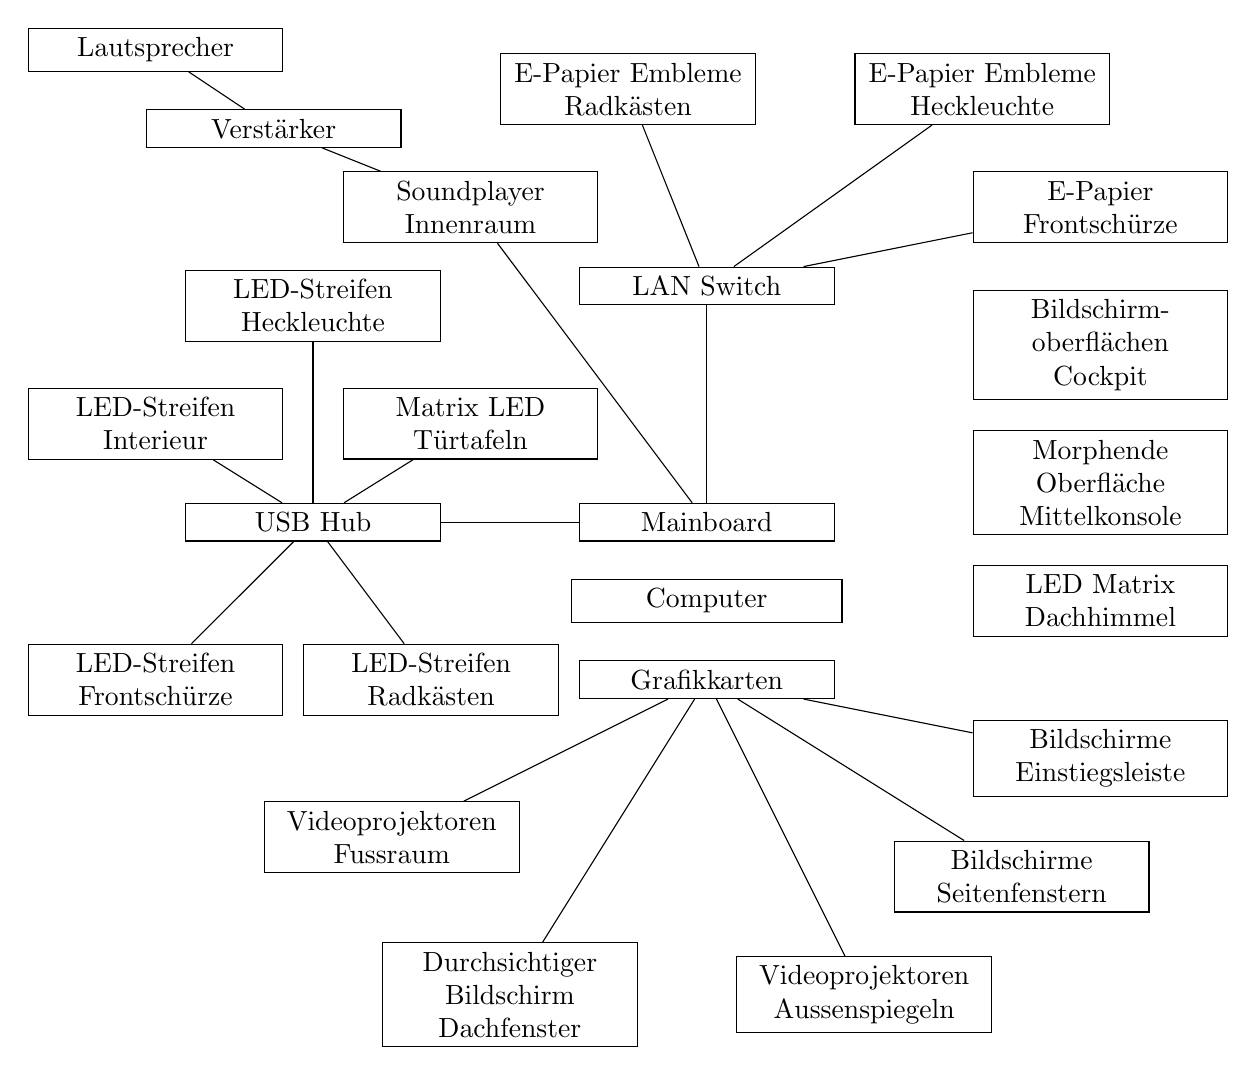
\begin{tikzpicture}
	\node[draw, rectangle, text width=3.2cm, align=center] (Computer) at (0, -1) {Computer};
	\node[draw, rectangle, text width=3cm, align=center] (Mainboard) at (0, 0) {Mainboard};
	\node[draw, rectangle, text width=3cm, align=center] (Grafikkarten) at (0, -2) {Grafikkarten};
	\node[draw, rectangle, text width=3cm, align=center] (LAN Switch) at (0, 3) {LAN Switch};
	\node[draw, rectangle, text width=3cm, align=center] (E-Papier Frontschürze) at (5, 4) {E-Papier Frontschürze};
	\node[draw, rectangle, text width=3cm, align=center] (LED-Streifen Frontschürze) at (-7, -2) {LED-Streifen Frontschürze};
	\node[draw, rectangle, text width=3cm, align=center] (E-Papier Embleme Radkästen) at (-1, 5.5) {E-Papier Embleme Radkästen};
	\node[draw, rectangle, text width=3cm, align=center] (LED-Streifen Radkästen) at (-3.5, -2) {LED-Streifen Radkästen};
	\node[draw, rectangle, text width=3cm, align=center] (Videoprojektoren Aussenspiegeln) at (2, -6) {Videoprojektoren Aussenspiegeln};
	\node[draw, rectangle, text width=3cm, align=center] (Bildschirme Seitenfenstern) at (4, -4.5) {Bildschirme Seitenfenstern};
	\node[draw, rectangle, text width=3cm, align=center] (LED-Streifen Heckleuchte) at (-5, 2.75) {LED-Streifen Heckleuchte};
	\node[draw, rectangle, text width=3cm, align=center] (E-Papier Embleme Heckleuchte) at (3.5, 5.5) {E-Papier Embleme Heckleuchte};
	\node[draw, rectangle, text width=3cm, align=center] (LED-Streifen Interieur) at (-7, 1.25) {LED-Streifen Interieur};
	\node[draw, rectangle, text width=3cm, align=center] (Matrix LED Türtafeln) at (-3, 1.25) {Matrix LED Türtafeln};
	\node[draw, rectangle, text width=3cm, align=center] (Bildschirme Einstiegsleiste) at (5, -3) {Bildschirme Einstiegsleiste};
	\node[draw, rectangle, text width=3cm, align=center] (Videoprojektoren Fussraum) at (-4, -4) {Videoprojektoren Fussraum};
	\node[draw, rectangle, text width=3cm, align=center] (Morphende Oberfläche Mittelkonsole) at (5, 0.5) {Morphende Oberfläche Mittelkonsole};
	\node[draw, rectangle, text width=3cm, align=center] (Durchsichtiger Bildschirm Dachfenster) at (-2.5, -6) {Durchsichtiger Bildschirm Dachfenster};
	\node[draw, rectangle, text width=3cm, align=center] (LED Matrix Dachhimmel) at (5, -1) {LED Matrix Dachhimmel};
	\node[draw, rectangle, text width=3cm, align=center] (Bildschirmoberflächen Cockpit) at (5, 2.25) {Bildschirm-oberflächen Cockpit};
	\node[draw, rectangle, text width=3cm, align=center] (Soundplayer Innenraum) at (-3, 4) {Soundplayer Innenraum};
	\node[draw, rectangle, text width=3cm, align=center] (USB Hub) at (-5, 0) {USB Hub};
	\node[draw, rectangle, text width=3cm, align=center] (Verstärker) at (-5.5, 5) {Verstärker};
	\node[draw, rectangle, text width=3cm, align=center] (Lautsprecher) at (-7, 6) {Lautsprecher};
	\draw (Mainboard) -> (LAN Switch);
	\draw (Mainboard) -> (Soundplayer Innenraum);
	\draw (Mainboard) -> (USB Hub);
	\draw (Grafikkarten) -> (Bildschirme Seitenfenstern);
	\draw (Grafikkarten) -> (Bildschirme Einstiegsleiste);
	\draw (Grafikkarten) -> (Videoprojektoren Fussraum);
	\draw (Grafikkarten) -> (Videoprojektoren Aussenspiegeln);
	\draw (Grafikkarten) -> (Durchsichtiger Bildschirm Dachfenster);
	\draw (LAN Switch) -> (E-Papier Frontschürze);
	\draw (LAN Switch) -> (E-Papier Embleme Radkästen);
	\draw (LAN Switch) -> (E-Papier Embleme Heckleuchte);
	\draw (USB Hub) -> (LED-Streifen Frontschürze);
	\draw (USB Hub) -> (LED-Streifen Radkästen);
	\draw (USB Hub) -> (LED-Streifen Heckleuchte);
	\draw (USB Hub) -> (LED-Streifen Interieur);
	\draw (USB Hub) -> (Matrix LED Türtafeln);
	\draw (Soundplayer Innenraum) -> (Verstärker);
	\draw (Verstärker) -> (Lautsprecher);
\end{tikzpicture}